\documentclass[thesis=M,english,hidelinks]{FITthesis}[2012/10/20]

\usepackage[utf8]{inputenc} % LaTeX source encoded as UTF-8
\usepackage{graphicx} % graphics files inclusion
\usepackage{dirtree} % directory tree visualisation
\usepackage[printonlyused]{acronym} % acronims
\usepackage{float} % floats
%\usepackage{indentfirst} % indent in first paragraph
\raggedbottom
%\usepackage[all]{hypcap} % for going to the top of an image when a figure reference is clicked
\usepackage[numbers]{natbib}
\usepackage{listings} % for the source code
\lstset{language=Python, frame=tb, basicstyle=\small} %or \small or \footnotesize etc.}


\graphicspath{{img/}} % images folder

\department{Department of Applied Mathematics}
\title{Multi-instrument music transcription}
\authorGN{Yevhen} %author's given name/names
\authorFN{Kuzmovych} %author's surname
\author{Yevhen Kuzmovych} %author's name without academic degrees
\authorWithDegrees{Bc. Yevhen Kuzmovych} %author's name with academic degrees
\supervisor{Ing. Marek Šmíd, Ph.D.}
\acknowledgements{THANKS (remove entirely in case you do not with to thank anyone)}
\abstractEN{Summarize the contents and contribution of your work in a few sentences in English language.}
\abstractCS{V n{\v e}kolika v{\v e}t{\' a}ch shr{\v n}te obsah a p{\v r}{\' i}nos t{\' e}to pr{\' a}ce v {\v c}esk{\' e}m jazyce.}
\placeForDeclarationOfAuthenticity{Prague}
\keywordsCS{Replace with comma-separated list of keywords in Czech.}
\keywordsEN{Replace with comma-separated list of keywords in English.}
\declarationOfAuthenticityOption{1} %select as appropriate, according to the desired license (integer 1-6)
% \website{http://site.example/thesis} %optional thesis URL


\begin{document}

%%%%%%%%%%%%%%%%%%%%%%%%%%%%% Custom commands %%%%%%%%%%%%%%%%%%%%%%%%%%%%%

\newcommand{\smplimage}[3][1]{
\centerline{\includegraphics[width=#1\textwidth]{#2.#3}}
}

% Usage:
%    \image[size]{diagram and lable name}{extention}{caption}
%    \image[1.3]{component_diagram}{pdf}{Component diagram}
\newcommand{\image}[4][1]{
\begin{figure}[H]
	\smplimage[#1]{#2}{#3}
	\caption{#4}
	\label{fig:#2}
\end{figure}
}


\newcommand{\class}[1]{\textit{\mbox#1}}
\newcommand{\method}[1]{\textit{\mbox#1}}
\newcommand{\field}[1]{\textit{\mbox#1}}
\newcommand{\app}[1]{\textit{\mbox#1}}
\newcommand{\file}[1]{\textit{\mbox#1}}
\newcommand{\bash}[1]{\textit{\mbox#1}}
\newcommand{\module}[1]{\textit{\mbox#1}}

\newcommand{\m}[1]{\mbox{#1}}

\newcommand{\definition}[1]{\textit{\textbf{\mbox{#1}}}}
%%%%%%%%%%%%%%%%%%%%%%%%%%%%%%%%%%%%%%%%%%%%%%%%%%%%%%%%%%%%%%%%%%%%%%%%%%%%


\setsecnumdepth{part}
\chapter{Introduction}\label{ch:introduction}
\chapter{Introduction}\label{ch:introduction}


\section{Problem definition}\label{sec:problem-definition}



The difficulty of multiple-F0 estimation lies in the fact that sound sources often overlap in time as well as in frequency. The extracted information is partly ambiguous.
Above all, when musical notes are played in harmonic relations, the partials of higher
notes may overlap completely with those of lower notes. Besides, spectral characteristics of musical instrument sounds are diverse, which increases the ambiguity in the
estimation of partial amplitudes of sound sources. The resulting complexity causes
not only octave ambiguity but also the ambiguity in the estimation of the number of
sources.


\section{Tuning}\label{sec:tuning}
\section{Sound envelope}\label{sec:sound-envelope}


\setsecnumdepth{all}
\chapter{State-of-the-art}\label{ch:state-of-the-art}
\chapter{State-of-the-art}\label{ch:state-of-the-art}

This chapter discusses existing state-of-the-art solutions for music transcription.

Sound transcription into sheet music is a combination of several techniques that include but not limited to source
instruments separation, pitch/note detection, event detection, etc.

Source separation and sound transcription to sheet music are fairly independent processes so their description and
approaches may come from different sources and different projects. Therefore, implementation will also be separated.

\section{Source separation}\label{sec:source-separation}

There were many successful attempts for music score source separation\cite{spleeter2019,singing-voice-separation,singing-voice-separation-article}.
Performance of such projects are commonly measured according to \textit{\ac{SiSeC}}\cite{stter20182018}
on the standard \textit{musdb18}\cite{musdb18} and \textit{DSD100}\cite{SiSEC16} datasets.

Latest and most successful project in this field is \textit{Spleeter}\cite{spleeter2019}. It is a project of
Deezer\footnote{Deezer is a French online music streaming service (deezer.com).}. It takes similar approaches to previous solutions
by University of London and Spotify\cite{singing-voice-separation}. Spleeter's pre-trained models will be used in the
module responsible for music source separation described in detail in the chapters~\ref{ch:analysis-and-design} and~\ref{ch:implementation}.

Following approaches are described in~\cite{spleeter2019,singing-voice-separation,singing-voice-separation-article}.

\subsection{Spleeters approach}\label{subsec:music-source-separation:approach}
The pre-trained models are U-nets\cite{singing-voice-separation} and follow similar specifications as in
\textit{Singing voice separation: a study on training data}\cite{singing-voice-separation-article}. The U-net is a
encoder/decoder \ac{CNN} architecture with skip connections\cite{spleeter2019}. Architecture used in this approach
showed a state-of-the-art results on DSD100 dataset\cite{singing-voice-separation} and in the last \ac{SiSeC}\cite{SiSEC16}.

\subsection{U-net architecture}\label{subsec:music-source-separation:u-net-architecture}
The U-Net shares the same architecture (shown on \cref{fig:u-net-architecture}) as a convolutional autoencoder with
extra skip-connections that bring back detailed information lost during the encoding stage to the decoding stage. It has
five strided\footnote{Transposed convolutions – also called \textit{fractionally strided convolutions} – work by
swapping the forward and backward passes of a convolution. One way to put it is to note that the kernel defines
a convolution, but whether it’s a direct convolution or a transposed convolution is determined by how the forward and
backward passes are computed.\cite{dumoulin2016guide}} 2D convolution layers in the encoder and five strided 2D
deconvolution layers in the decoder.

The goal of the neural network architecture is to predict the vocal and instrumental components of its input indirectly:
the output of the final decoder layer is a soft mask for each source that is multiplied element-wise with the mixed
spectrogram to obtain the final estimate.

\image{u-net-architecture}{pdf}{Network Architecture\cite{singing-voice-separation}}

\pagebreak

\subsection{Data and training}\label{subsec:music-source-separation:data-and-training}

Spleeter's training dataset is an internal Deezer's dataset and is not shared (for copyright reasons).

Another project with similar approach, as explained in the dedicated article\cite{singing-voice-separation-article},
uses two datasets during training of the models: \textit{MUSDB}\cite{musdb18} and \textit{Bean}(private dataset).

\textit{MUSDB} is the largest and most up-to-date public dataset for source separation\cite{musdb18}. It contains 150
songs of western music genres primarily pop/rock, some hip-hop, rap and metal songs. And each song consists of four
audio tracks: drums, bass, vocal and other. Original mix (and input of the model) is produced by summing tracks of four
sources (expected outputs) together.


\section{Multi-pitch Detection}\label{sec:multi-pitch-detection}
There were several projects utilizing different approaches to a problem of \ac{AMT}. Following section discuss these
approaches and projects that used them.

The most important part of transcription of sound into sheet music is pitch (and subsequently note) detection. The core
problem of polyphonic music transcription is multi-pitch detection.

In his Ph.D.\ research \textit{Multiple fundamental frequency estimation of polyphonic recordings}\cite{fundamental-frequency-estimation},
Chunghsin Yeh classifies multi-pitch detection systems according to their estimation type into two categories: joint and
iterative. The \textit{iterative} approach extracts the most eminent frequency per each iteration, until no other pitch
can be estimated and extracted. Commonly, iterative estimators generate errors on each iteration but are much cheaper in
terms of computation costs.

On the other side, the \textit{joint} estimation models evaluate combinations of pitches at once, which leads to
increase in accuracy but also in computation costs. Most of the latest approaches and state-of-the-art solutions fall
into joint category. Solution in this thesis also follows this category and will be discussed in detail in \cref{ch:analysis-and-design}.

\subsection{Feature-based multi-pitch detection}\label{subsec:feature-based-multi-pitch-detection}
Most multi-pitch estimation and note tracking approaches exploit methods that come from signal processing. There is no
specific model (\ac{ML} or other), and notes are detected using audio features that come from the input time-frequency
representation (spectrogram) either in an iterative or joint way. Usually, multi-pitch estimation uses a \textit{pitch
candidate set score function} or a \textit{pitch salience function}.

A \textit{salience function} is a function that provides an estimation of the predominance of different frequencies in
an audio signal at every time frame\cite{pitch-salience-function}. A \textit{pitch candidate set score function} is
function designed to evaluate the plausibility of the combination of the hypothetical sources\cite{fundamental-frequency-estimation}.

These feature-based techniques have produced the best results in the \ac{MIREX} multi-pitch and note tracking
evaluations. The work by Chunghsin Yeh\cite{fundamental-frequency-estimation} was the best performing method in
the \ac{MIREX} multi-pitch and note tracking tasks. Yeh proposed a joint pitch estimation algorithm based on a pitch
candidate set score function. Having a set of pitch candidates, the overlapping partials are detected and smoothed
according to the spectral smoothness principle, which states that the spectral envelope\footnote{\textit{Spectral
envelope} of the sound determines the particular vowel sound produced, and is, in general, one of the important acoustic
features that determine its perceived timbre\cite{kumar2007hierarchical}.} of a musical sound tends to be slowly
changing as a function of frequency. The score function for the pitch candidate set consists of four features:
harmonicity, mean bandwidth, spectral centroid, and ``synchronicity'' (synchrony). A polyphony inference mechanism based
on the score function increase selects the optimal pitch candidate set\cite{fundamental-frequency-estimation}.

In the following year, the best performing method for the \ac{MIREX} multi-pitch estimation and note tracking tasks,
Karin Dressler described in her work \textit{Multiple fundamental frequency extraction for MIREX}\cite{dressler2012multiple}.
A multiresolution \ac{FFT} (see \cref{subsec:multiresolution-fft} on multiresolution \ac{FFT}) analysis was used as
an input time/frequency representation, where the magnitude for each spectral bin was multiplied with the bin’s
instantaneous frequency. Pitch estimation is made by identifying spectral peaks and performing pair-wise analysis on
them, resulting on ranked peaks according to harmonicity, smoothness, the appearance of intermediate peaks, and harmonic
number. Finally, the system tracks tones over time using an adaptive magnitude and a harmonic magnitude threshold.

Other notable feature-based \ac{AMT} solution was introduced in the work by Pertusa and Inesta \textit{Multiple
fundamental frequency estimation using Gaussian smoothness and short context}\cite{pertusa2008multiple}. They proposed
a computationally inexpensive method for multi-pitch detection which computes a pitch salience function and evaluates
combinations of pitch candidates using a measure of distance between a \ac{HPS} and a smoothed \ac{HPS}. Another
approach for feature-based \ac{AMT} was proposed in \textit{Hybrid genetic algorithm based on gene fragment competition
for polyphonic music transcription}\cite{reis2008hybrid}, which uses genetic algorithms for estimating a transcription
by mutating the solution until it matches a similarity criterion between the original signal and the synthesized
transcribed signal.

More recently, Peter Grosche et al. proposed\cite{grosche2012automatic} an \ac{AMT} method based on a mid-level
representation derived from a multiresolution \ac{FFT} combined with an instantaneous frequency estimation. His system
also combines event (specifically start of the note) detection and tuning estimation for computing predictions. Finally,
Juhan Nam et al. proposed\cite{nam2011classification} a classification-based approach for piano transcription using
features learned from deep belief networks\cite{humphrey2013feature} for computing a mid-level time-pitch representation.

\subsection{Statistical model-based multi-pitch detection}\label{subsec:statistical-model-based-multi-pitch-detection}
Many approaches in the literature formulate the multi-pitch estimation problem within a statistical framework. As
Valentin Emiya et al. explains in their article \textit{Multipitch Estimation of Piano Sounds Using a New Probabilistic
Spectral Smoothness Principle}\cite{proba-spectral-smoothness}: given an observed frame $\pmb{x}$ and a set $\pmb{C}$ of
all possible fundamental frequency combinations, the frame-based multi-pitch estimation problem can then be viewed as
a \ac{MAP} estimation problem:

\[ \hat{C}_{MAP} = \argmax_{C \in \pmb{C}} P(C|\pmb{x}) = \argmax_{C \in \pmb{C}} \frac{P(\pmb{x}|C)P(C)}{P(\pmb{x})} \]

where $C = \{F_0^1, \dots, F_0^N\}$ is a set of possible frequencies (considering tuning of an instrument), $\pmb{C}$ is
the set of all possible $F_0$ combinations, and $\pmb{x}$ is the observed audio signal within a single analysis frame.

An example of \ac{MAP} estimation-based transcription is the \textit{PreFEst} system introduced by Masataka Goto in his
article \textit{A real-time music-scene-description system: predominant-F0 estimation for detecting melody and bass
lines in real-world audio signals}\cite{predominant-f0-estimation}, where each harmonic is modelled by a Gaussian
centered at its position on the log-frequency axis. \ac{EM} algorithm is used to estimate \ac{MAP} value.
An extension of this method was proposed by Kameoka et al. in \textit{A Multipitch Analyzer Based on Harmonic Temporal
Structured Clustering}\cite{harmonic-temporal-structured-clustering}, which jointly estimates multiple possible
frequencies, moments of start and end of the note, and dynamics. Partials are modelled using Gaussians placed at
the positions of partials in the log-frequency domain and the synchronous evolution of partials belonging to the same
source is modelled by Gaussian mixtures.

More recently, Peeling and Godsill, in their article \textit{Multiple pitch estimation using non-homogeneous Poisson
processes}\cite{peeling2011multiple}, also proposed a likelihood function for multiple-pitch estimation where for a
given time frame, the occurrence of peaks in the frequency domain is assumed to follow an inhomogeneous Poisson process.
Also, Koretz and Tabrikian in \textit{Maximum a posteriori probability multiple-pitch tracking using the harmonic
model}\cite{koretz2011maximum}, proposed an iterative method for multi-pitch estimation, which combines \ac{MAP} and
\ac{ML} criteria. The predominant source is expressed using a harmonic model while the remaining harmonic signals are
modelled as Gaussian interference sources\cite{koretz2011maximum}.

\pagebreak

\subsection{Spectrogram factorisation-based multi-pitch detection}\label{subsec:spectrogram-factorisation-based-multi-pitch-detection}
The majority of recent multi-pitch detection papers utilise and expand spectrogram factorisation techniques. \ac{NMF} is
a technique first introduced in their paper by Paris Smaragdis et al.\ \cite{smaragdis2003non} as a tool for music
transcription. In its simplest form, the \ac{NMF} model decomposes an input spectrogram
$\pmb{X} \in \mathbb{R}^{K \times N}_+$ with $K$ frequency bins and $N$ frames: \[ \pmb{X} \approx \pmb{WH} \]
where $R \ll K, N$; $\pmb{W} \in \mathbb{R}^{K \times R}_+$ contains the spectral bases for each of the $R$ pitch
components; and $\pmb{H} \in \mathbb{R}^{R \times N}_+$ is the pitch activity matrix across time.

In his paper \textit{Realtime multiple pitch observation using sparse non-negative constraints}, Cont Arshia applies
\ac{NMF} to \ac{AMT} problem. Sparseness constraints were added into the \ac{NMF} update rules, in order to find
meaningful transcriptions using a minimum number of non-zero elements in $\pmb{H}$. Emmanuel Vincent et al. in their
article \textit{Adaptive harmonic spectral decomposition for multiple pitch estimation}\cite{vincent2009adaptive}
incorporated harmonicity constraints in the \ac{NMF} model, resulting in two algorithms: harmonic and inharmonic
\ac{NMF}. The inharmonic version of the algorithm is also able to support deviations from perfect harmonicity and
standard equal temperament tuning. Also, Nancy Bertin et al. in their article\cite{bertin2010enforcing} proposed
a Bayesian framework for \ac{NMF}, which considers each pitch as a model of Gaussian components in harmonic positions.

More recently, Ochiai et al. in his paper \textit{Explicit beat structure modeling for non-negative matrix
factorization-based multipitch analysis}\cite{ochiai2012explicit} proposed an algorithm for multi-pitch detection and
beat structure analysis. The \ac{NMF} objective function is constrained using information from the rhythmic structure of
the recording. It helped to improve transcription accuracy in highly repetitive recordings.

This thesis approaches \ac{AMT} problem in similar fashion to spectrogram factorisation and feature-based methods.
Detailed description of used methods is in \cref{ch:analysis-and-design}.

\section{Note Tracking}\label{sec:note-tracking}

Typically \ac{AMT} algorithms compute a time-pitch representation which needs to be further processed in order to detect
note events with a discrete pitch value, a time of start and end of the note. This process is called \textit{note
tracking}. Most spectrogram factorisation-based methods estimate the binary piano-roll representation from the pitch
activation matrix using simple thresholding (i.e.\ in \textit{Explicit beat structure modeling for non-negative matrix
factorization-based multipitch analysis}\cite{grindlay2011transcribing} by Graham Grindlay and in \textit{Adaptive
harmonic spectral decomposition for multiple pitch estimation}\cite{vincent2009adaptive} by Emmanuel Vincent). This
approach will be used in the implementation of the thesis. Also, one simple and fast optimisation for note tracking is
minimum duration pruning, which is applied after thresholding (idea comes from paper by Arnaud Dessein et al.
\textit{Real-time polyphonic music transcription with non-negative matrix factorization and beta-divergence}\cite{dessein2010real}).
Primary idea is that output notes that have a duration smaller than a predefined threshold are removed from the final
score. Similar method was also used by Juan Pablo Bello et al. in their paper \textit{Automatic piano transcription
using frequency and time-domain information}\cite{bello2006automatic}, where more complex rules for note tracking were
used, addressing cases such as where a small gap exists between two note events. This method will also be applied as it
is easy to implement.

For threshold based method, there are several issues that may appear for different instruments, primarily related to how
notes are used and written for them in practice. For instance, for percussion instruments, note decay is exponential and
physical duration of the note is irrelevant as it is not controlled(for most percussion instruments) by a musician. so
notes may appear short and require pauses(rests) after them, even though they (rests) would not be written in sheet
music. Such problems may be solved with other rule based solutions specific to each instrument that requires them or
more complex approaches. Even though, in frameworks of this thesis, simple threshold-based solution was used for
the note tracking task, it is important to know other approaches for this problem.

There were several more complex solutions applied to the problem of note tracking. Following are some of them, though
without detailed description of the approach.

\acp{HMM} are frequently used at a stage of postprocessing of note tracking. In his work \textit{A discriminative model
for polyphonic piano transcription}\cite{poliner2006discriminative}, Graham Poliner proposes a note tracking method that
utilizes pitch-wise \acp{HMM}, where each \ac{HMM} has two states, indicating note activity and inactivity. \ac{HMM}
parameters (state transitions and priors) were learned directly from a ground-truth training set, while the observation
probability is given by the posteriogram output for a specific pitch.

In \textit{Polyphonic music transcription using note event modeling}\cite{ryynanen2005polyphonic} by Matti P Ryynanen
and Anssi Klapuri, a feature-based multi-pitch detection system was combined with a musicological model for estimating
musical key and note transition probabilities. Note events are described using 3-state \acp{HMM}, which model
the envelope (attack, sustain, and noise/silence states) of each sound. In addition, context-dependent \acp{HMM} were
employed in \textit{Automatic transcription of recorded music}\cite{grosche2012automatic} for determining note events by
combining the output of a multi-pitch detection system with an note-start detection system.

Finally, \acp{DBN} were proposed by Shigeki Sagayama et al. in their paper\cite{raczynski2009note} for note tracking.
They used the pitch activation of an \ac{NMF}-based multi-pitch detection algorithm as input. The \ac{DBN} has a note
layer in the lowest level, followed by a note combination layer. Model parameters were learned using MIDI files from
F. Chopin piano pieces.

\section{Tuning, time signature, key, and tempo estimation}\label{sec:other-amt-subtasks}
There are several other subtasks of \ac{AMT} systems that have to be resolved to be able to generate correct
transcription in a form of sheet music. Also, such estimates, if properly incorporated to the system, may improve
estimates of detected pitches and their durations, events. Tuning, time signature, key, and tempo estimation are such
tasks.

\subsection{Key and chord detection}\label{subsec:key-and-chord-detection}
Most Western music has a harmonic organisation around one key. The key is generally unchanged over whole, or at least
sections of musical pieces. At one point in time, the harmony may be described by chord, which is a combinations of
simultaneous or sequential notes which are perceived to belong together (and in general sound nice together, even though
any combination of notes has its chord). Algorithms for key (and similarly for chord) detection use template matching or
\acp{HMM}. For key detection, this theses uses the simple approach defined in \cref{sec:key-classification}.

\subsection{Tempo and time signature estimation}\label{subsec:tempo-and-time-signature-estimation}
The \textit{beats} are regularly spaced in time pulses. They are the primary unit that defines tempo and rhythm of most
Western music. A number of beats per unit of time (commonly per minute in sheet music) define \textit{tempo}. A number
of beats per uniform repetitive sections in score (bars) define \textit{time signature}. In order to interpret an audio
recording in terms of such a structure (which is necessary in order to produce Western music notation), the first step
is to determine the rate of the most salient pulse, which is the tempo.

Algorithms used for tempo induction include autocorrelation, Fourier transforms, and periodicity transform, which are
applied to audio features such as a note-start detection function (as Fabien Gouyon and Simon Dixon describe in their
article \textit{A review of automatic rhythm description systems}\cite{gouyon2005review}). The next step involves
estimating the timing of the beats constituting the main pulse, a task known as beat tracking. Again, numerous
approaches have been proposed, such as rule-based methods (as in \textit{Computational models of beat induction:
The rule-based approach}\cite{desain1999computational} by Peter Desain and Henkjan Honing), adaptive oscillators (as
in \textit{Resonance and the perception of musical meter}\cite{large1994resonance} by Edward W Large and John F Kolen),
agent-based or multiple hypothesis trackers (as in \textit{Automatic extraction of tempo and beat from expressive
performances}\cite{dixon2001automatic} by Simon Dixon), and other. The final step for rhythmic analysis consists of
estimating the time signature, which indicates how beats are grouped and subdivided at respectively higher and lower
metrical levels, and assigning each note-start and offset time to a position in this structure\cite{cemgil2011monte}.



\chapter{Analysis and design}\label{ch:analysis-and-design}
\chapter{Analysis and design}\label{ch:analysis-and-design}

This chapter defines architecture of the chosen solution. It provides details of used approaches for music sources
separation and models used in it, pitch extraction and signal analysis, event detection, etc.

\section{Architecture}\label{sec:architecture}

The implementation of the system is separated into logical parts responsible for sound data streaming, music source
separation, pitch and events detection, transcription and score generation. Following diagram shows architecture of
the solution. Arrows represent data flow. Dotted arrows represent flow that is optional. If given parameters (like
tuning, tempo, time signature and key) are specified by user, they are not being estimated. Each rectangular block
represents logical module in implementation.

Detailed description of each component is in the dedicated section following the diagram.

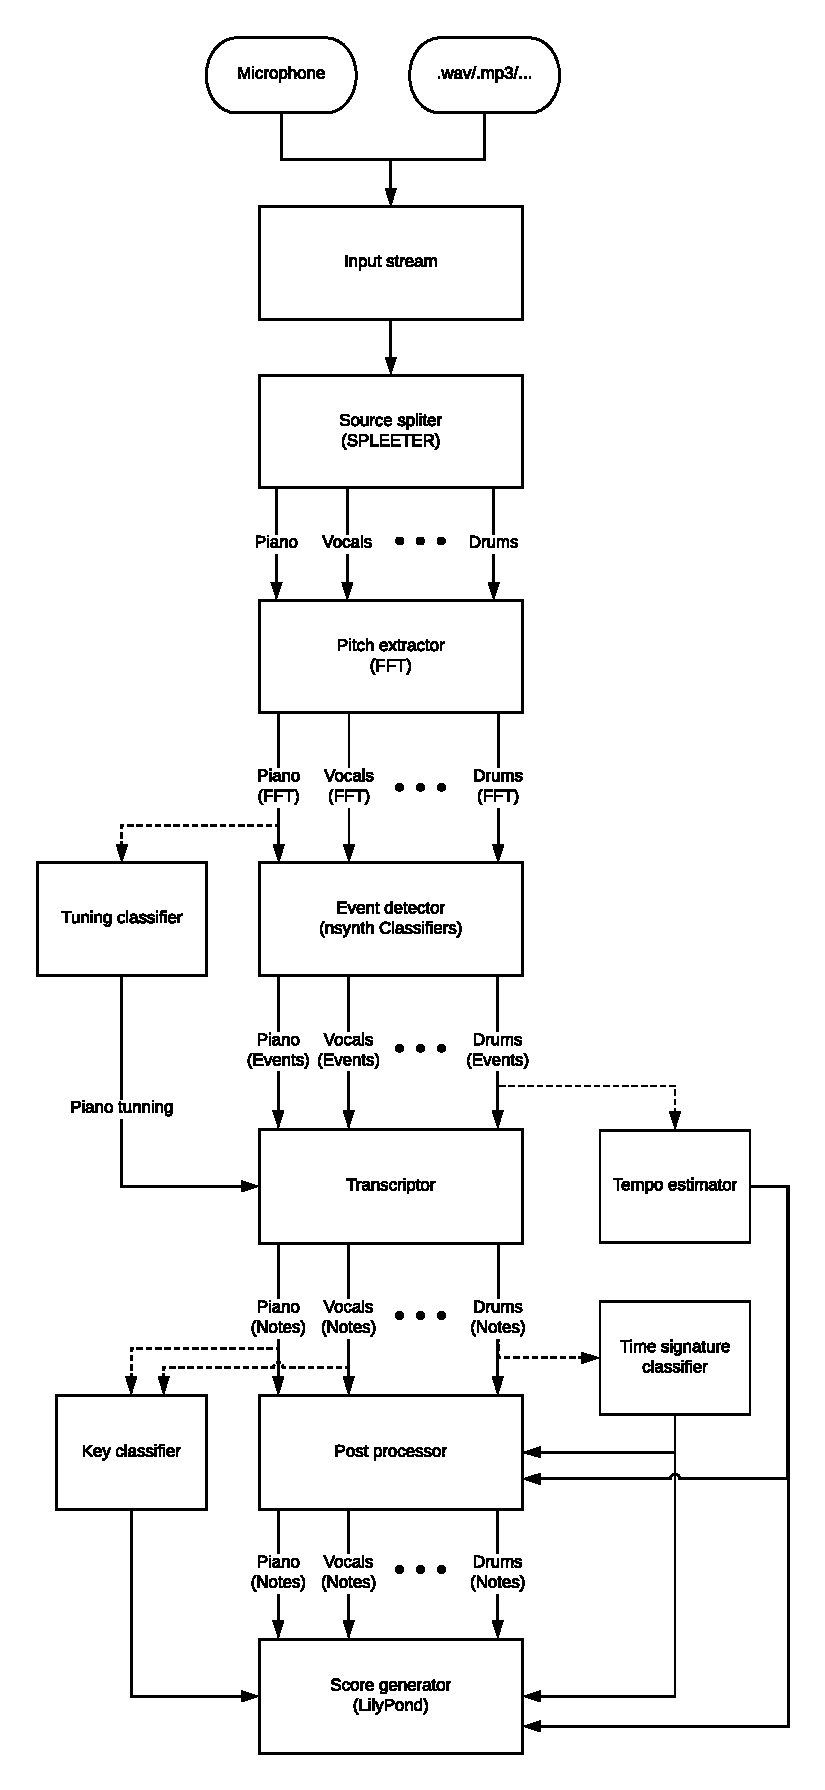
\includepdf{architecture.pdf}

\section{Audio streaming}\label{sec:audio-streaming}

This implementation directly works only with \ac{WAVE} (.wav/.wave). Any other format is converted to WAVE first,
then processed.

\subsection{WAVE format}\label{subsec:wave-format}
\textbf{WAVE} is an audio file format standard, developed by Microsoft and IBM, for storing an audio bitstream on PCs.
What's important for this thesis and implementation is that it stores data in chunks in \ac{LPCM} format. This format
allows to perform \ac{DFT} used in pitch extraction.

\subsection{Sampling rate}\label{subsec:sampling-rate}
\ac{LPCM} mentioned above stores sampled amplitude of recorded audio at specific sampling rate (frequency, measured in
Hz).

The most common sampling rate is 44.1 kHz, or 44100 samples per second. This is the standard for most consumer audio,
used for formats like CDs\cite{digital-audio-basics}.

The sampling rate determines the range of frequencies captured in digital audio. According to \textit{Nyquist Theorem},
a signal which has a Fourier transform having only frequencies upto a certain maximum $f_m$, we can obtain the analog
signal $f(t)$ from the sampled signal $f'(t)$ by passing the sampled signal $f'(t)$ through a low pass filter provided
that the sampling frequency $f_s$ is more than twice the maximum frequency $f_m$ present in the signal i.e.\ ,
$f_s > 2f_m$\cite{signals-and-systems}. Hence, having 44100 Hz sampling rate, we can reproduce and analise frequencies
up to 22050 Hz. The lowest frequency a person can hear is 20 Hz. The highest frequency humans can hear are in the range
of 20.000 Hz, but only young people can hear such high tones\cite{roots-of-modern-technology}.

The implementation is able to process input sound with any sampling rate, though lower sampling rates may cause
inaccuracies for high frequencies due to effect called \textit{aliasing}. The phenomenon of aliasing occurs if
the sampling rate is less than the Nyquist rate ($2\times$ the highest frequency). If sampling rate is less than or greater
than the Nyquist rate, it is called under sampling or over sampling. Aliasing phenomenon occurs only for under sampling.
If the sampling frequency is too low the frequency spectrum overlaps, and becomes corrupted\cite{signals-and-systems}.

\pagebreak

\section{Music source separation}\label{sec:music-source-separation}

First step of the sound processing is separation of the sound into source instruments (i.e.\ voice, guitar, piano,
etc.)

As was mentioned in previous chapter, for separation of source instruments, this implementation uses \textit{Spleeter}.
\textit{Spleeter} is a fast and state-of-the art music source separation tool with pre-trained
models\cite{spleeter2019}. Its implementation contains three pre-trained models:

\begin{itemize}
	\item vocals/accompaniment separation
	\item 4 stems separation as in \ac{SiSeC}\cite{stter20182018} (vocals, bass, drums and other)
	\item 5 stems separation with an extra piano stem (vocals, bass, drums, piano and other). It is, to the authors
	knowledge, the first released model to perform such a separation.
\end{itemize}

Estimations for all the models is performed in a frequency domain of the sound. Meaning that sound data from time domain
is converted to frequency domain using \ac{FFT}, passed to the models described in section~\ref{subsec:music-source-separation:u-net-architecture}
about U-net architecture. Output of the model is separated tracks for each instrument and voice. To get sound of each
instrument and voice in time domain (as it would be represented in \ac{WAVE}), we'd need to pass it through \ac{IDFT}.
Though it is unnecessary, as all the subsequent processing will be performed on the sound in frequency domain.

More about \ac{FFT} in the following section~\ref{sec:pitch-extraction} about pitch extraction.

\section{Pitch extraction}\label{sec:pitch-extraction}

\subsection{Multiresolution \ac{FFT}}\label{subsec:multiresolution-fft}
https://pdfs.semanticscholar.org/d55f/984d569786e1bbf945f7683361ffbbfff79a.pdf

\section{Event detection}\label{sec:event-detection}

\section{Tuning classification}\label{sec:tunning-classification}

\section{Transcription}\label{sec:transcription}

\section{Tempo estimation}\label{sec:tempo-estimation}

\section{Time signature estimation}\label{sec:time-signature-estimation}

\section{Key classification}\label{sec:key-classification}

\section{Post processing}\label{sec:post-processing}

\section{Score generation}\label{sec:score-generation}





\chapter{Realisation}\label{ch:realisation}
\chapter{Realisation}\label{ch:realisation}


\setsecnumdepth{part}
\chapter{Conclusion}\label{ch:conclusion}
\chapter{Conclusion}\label{ch:conclusion}

This thesis introduces a reader to the problem of automated transcription of a multi-instrument sound recording to
a sheet music. It discusses a state-of-the-art solutions to the tasks of a source instruments separation, pitch
detection, key and time signatures estimation, etc.

The goal has been reached at a sufficient level. The analysis and design of the implementation allows for future
expansion and improvement of quality of the processing pipeline.

\section{Possible improvements}\label{sec:possible-improvements}

Implementation does not take into consideration the \textit{dynamics} of the notes. Dynamic of a sound describes its
amplitude or loudness (\pp, \p, \mf, \f, \ff, etc.), its emotional intensity and change through time (crescendo,
decrescendo). It is often an inalienable part of the description of the generated sound, hence a part of the output
sheet music. The solution to this task could be simple rule based or more complex that utilize \ac{ML} or statistical
analysis.

Another optimization for pitch detection could be usage of \textit{Multiresolution \ac{FFT}}. This method is widely-used
in a field of \ac{MIR} tasks. The frequency components of a \ac{DFT} are equally spaced and have a constant resolution.
However, in polyphonic music a higher frequency resolution is needed in the low and mid frequencies where there is
a higher density of harmonics. On the other hand, frequency modulation gets stronger as the number of harmonic is
increased, requiring shorter windows for improved time resolution~\cite{cancela2009efficient}. Thus, a multi resolution
spectral representation is highly desired for the analysis of music signals and can be a great improvement for the pitch
detection module of this implementation.



\bibliographystyle{iso690}
\bibliography{bibliography}

\setsecnumdepth{all}
\appendix


\chapter{Acronyms}\label{ch:acronyms}
\begin{acronym}
\end{acronym}


\chapter{Contents of enclosed CD}\label{ch:contents-of-enclosed-cd}

%change appropriately

\begin{figure}
	\dirtree{%
		.1 readme.txt\DTcomment{the file with CD contents description}.
		.1 exe\DTcomment{the directory with executables}.
		.1 src\DTcomment{the directory of source codes}.
		.2 wbdcm\DTcomment{implementation sources}.
		.2 thesis\DTcomment{the directory of \LaTeX{} source codes of the thesis}.
		.1 text\DTcomment{the thesis text directory}.
		.2 thesis.pdf\DTcomment{the thesis text in PDF format}.
		.2 thesis.ps\DTcomment{the thesis text in PS format}.
	}
\end{figure}

\end{document}
